\documentclass[tikz,border=10pt]{standalone}
\usepackage[utf8]{inputenc}
\usepackage[T1]{fontenc}
\usepackage{amsmath,amssymb}
\usepackage{tikz}
\usetikzlibrary{shapes.geometric, arrows.meta, positioning, calc, fit, backgrounds}

\definecolor{primary}{HTML}{0F172A}
\definecolor{primaryblue}{HTML}{1E3A8A}
\definecolor{accentblue}{HTML}{0284C7}
\definecolor{tealaccent}{HTML}{0D9488}
\definecolor{darkgreen}{HTML}{065F46}
\definecolor{lightgreen}{HTML}{ECFDF5}
\definecolor{crimson}{HTML}{991B1B}
\definecolor{lightred}{HTML}{FEF2F2}
\definecolor{amber}{HTML}{B45309}
\definecolor{lightamber}{HTML}{FFFBEB}
\definecolor{boxbg}{HTML}{F8FAFC}

\begin{document}

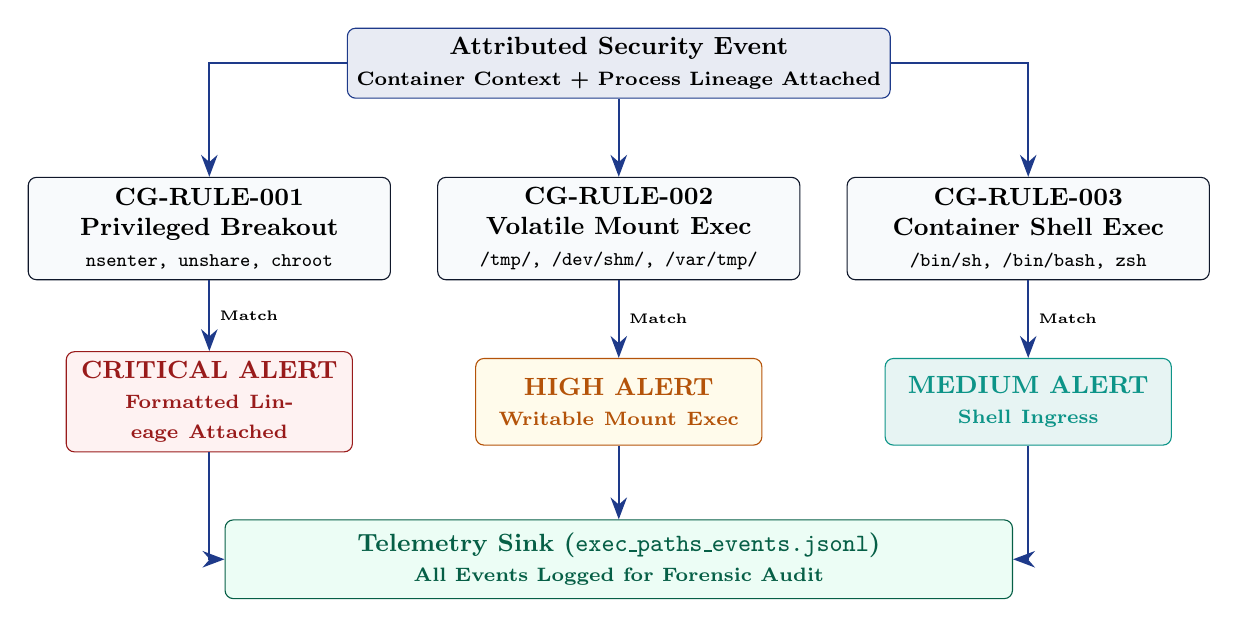
\begin{tikzpicture}[
    event/.style={rectangle, draw=primaryblue, fill=primaryblue!10, rounded corners=3pt, font=\small\bfseries, align=center, minimum width=6cm, minimum height=0.85cm},
    rule/.style={rectangle, draw=primary, fill=boxbg, rounded corners=3pt, font=\small\bfseries, align=center, minimum width=4.6cm, minimum height=1.3cm},
    crit/.style={rectangle, draw=crimson, fill=lightred, text=crimson, rounded corners=3pt, font=\small\bfseries, align=center, text width=3.4cm, minimum height=1.1cm},
    high/.style={rectangle, draw=amber, fill=lightamber, text=amber, rounded corners=3pt, font=\small\bfseries, align=center, text width=3.4cm, minimum height=1.1cm},
    med/.style={rectangle, draw=tealaccent, fill=tealaccent!10, text=tealaccent, rounded corners=3pt, font=\small\bfseries, align=center, text width=3.4cm, minimum height=1.1cm},
    pass/.style={rectangle, draw=darkgreen, fill=lightgreen, text=darkgreen, rounded corners=3pt, font=\small\bfseries, align=center, minimum width=10cm, minimum height=1.0cm},
    arrow/.style={-{Stealth[scale=1.2]}, thick, draw=primaryblue}
]
    \node[event] (ev) at (0, 3.5) {Attributed Security Event\\ \scriptsize Container Context + Process Lineage Attached};

    \node[rule] (r1) at (-5.2, 1.4) {\textbf{CG-RULE-001}\\ Privileged Breakout\\ \scriptsize\texttt{nsenter, unshare, chroot}};
    \node[rule] (r2) at (0.0, 1.4) {\textbf{CG-RULE-002}\\ Volatile Mount Exec\\ \scriptsize\texttt{/tmp/, /dev/shm/, /var/tmp/}};
    \node[rule] (r3) at (5.2, 1.4) {\textbf{CG-RULE-003}\\ Container Shell Exec\\ \scriptsize\texttt{/bin/sh, /bin/bash, zsh}};

    \node[crit] (a1) at (-5.2, -0.8) {\textbf{CRITICAL ALERT}\\ \scriptsize Formatted Lineage Attached};
    \node[high] (a2) at (0.0, -0.8) {\textbf{HIGH ALERT}\\ \scriptsize Writable Mount Exec};
    \node[med] (a3) at (5.2, -0.8) {\textbf{MEDIUM ALERT}\\ \scriptsize Shell Ingress};

    \node[pass] (sink) at (0, -2.8) {\textbf{Telemetry Sink (\texttt{exec\_paths\_events.jsonl})}\\ \scriptsize All Events Logged for Forensic Audit};

    \draw[arrow] (ev) -| (r1);
    \draw[arrow] (ev) -- (r2);
    \draw[arrow] (ev) -| (r3);

    \draw[arrow] (r1) -- node[right, font=\tiny\bfseries]{Match} (a1);
    \draw[arrow] (r2) -- node[right, font=\tiny\bfseries]{Match} (a2);
    \draw[arrow] (r3) -- node[right, font=\tiny\bfseries]{Match} (a3);

    \draw[arrow] (a1) |- (sink);
    \draw[arrow] (a2) -- (sink);
    \draw[arrow] (a3) |- (sink);
\end{tikzpicture}

\end{document}
